\section{Орбиты в моделях с ротационной симметрией}
~\par
Численное решение уравнений движения позволяет проанализировать свойства галактических орбит в реалистичных моделях галактик. При этом использование сложных моделей потенциалов не дает возможности аналитического решения уравнений движения, и орбиты звёзд приходится получать только путем их численного решения. Под \\textit{орбитой звезды} понимается орбита материальной точки единичной массы. Однако для многих задач необходимо получение параметров орбит звёзд и скоплений именно в реалистичных моделях. В качестве примера можно указать задачу о получении мест рождения звёздных скоплений, когда орбиты рассчитываются назад по времени на величину возраста скопления. С помощью анализа орбит исследуется возможность длительного существования движущихся групп звёзд.\\

Задавая самые различные значения скоростей звёзд в начальный момент времени, что соответствует заданию разных значений интегралов движения, можно получать самые различные орбиты, а так же проводить их классификацию их форм. Подобное изыскание провел Оллонгрен~\cite{OLLONGREN}. Он установил, что оказалось удобным рассматривать движение точек, изображающих звёзды, в сопутствующей меридиональной плоскости, т.е. в плоскости, проходящей через ось вращения Галактики и вращающейся вокруг этой оси симметрии вместе с рассматриваемой точкой. В этом случае мы фактически рассматриваем движение точки в плоскости (R, z). Также им было установлено, что большинство орбит реальных звёзд в Галактике - ящичные.\\

Мы будем различать понятия <<траектория>> и <<орбита>>. \text{Траектория --} это непрерывная линия, которую фактически описывает движущееся тело (звезда, материальная точка) по отношению к заданной системе отсчета. За конечный интервал времени траектория приобретает конечную длину. Орбита --- это потенциально возможная траектория на (полу)бесконечном интервале времени, соответсвующая данному полю сил и начальным (краевым) условиям. Траекторию можно наблюдать, а орбиту рассчитывать \emph{a priori}. Например, для кеплерова движения барицентрические орбиты являются коническими сечениями, а траектории --- их дугами. Возможно многократное покрытие орбиты траекторией~\cite{KutuzovOssipkov}.\\

\subsection{Уравнения движения}
~\par
Для расчета орбит будем решать задачу Коши, в которой система обыкновенных дифференциальных уравнений в общем случае имеет вид:

\begin{equation}\label{zK}
\ddot{\textbf{r}} = \nabla \varphi, \qquad \textbf{r}(t_0)=\textbf{r}_0,\, \textbf{v}(t_0)=\textbf{v}_0,
\end{equation}
где $\textbf{r}$~--- радиус-вектор пробной звезды, $\textbf{v}$~--- вектор скорости, $\nabla$~--- векторный оператор набла.
$$
\textbf{r} = (R, \theta, z)^T, \quad
\nabla = \left( \frac{\partial}{\partial R}, \frac{1}{R}\frac{\partial}{\partial \theta}, \frac{\partial}{\partial z} \right)^T
$$

Для стационарной ротационно-симметричной модели имеют место интегралы энергии $ E $ и площадей $ I $~\cite{ogor}

\begin{equation}\label{EI}
E = \frac{1}{2}(v_R^2 + v_z^2 + v_{\theta}^2) - \varphi(\xi) , \quad
I = R v_{\theta}
\end{equation}
где $v_R, v_{\theta}, v_z$~--- компоненты скорости соответствующих цилиндрических координат $R, \theta, z$.
Тогда задача сводится к решению системы шести обыкновенных дифференциальных уравнений. Благодаря интегралам энергии $E$ и площадей $I$ получаем систему, состоящую из 5 дифференциальных уравнений~\cite{KutuzovOssipkov}:

\begin{equation}\label{systRz}
\left\{ \begin{aligned}
&\dot R = \, v_R, & \, \dot v_R & = \frac{I^2}{R^3} + \frac{\partial \varphi }{\partial R },\\
&\dot \theta = \, \frac I{R^2}, & , \dot v_z & = \frac{\partial \varphi}{\partial z },\\
&\dot z = \, v_z. &
\end{aligned}
\right.
\end{equation} 

\subsection{Выбор метода численного интегрирования}

Вычисления ведутся в среде {\ttfamily Maple 13 (x64)}, {\ttfamily Build ID: 397624}. Используемый метод интегрирования: метод Рунге-Кутта-Фельберга (RKF45).\\
%{ttfamily
%\begin{verbatim}
%dsolve({sys,
% R(0)=R0, Th(0)=Th0, Z(0)=z0, vR(0)=vR0, vz(0)=vz0},
% fncs,
% numeric,
% method = rkf45,
% output = listprocedure):
%\end{verbatim}
%}

Метод Рунге-Кутта-Фельберга 4-го порядка (Fehlberg 4(5)) был предложен немецким математиком Эрвином Фельбергом (Erwin Fehlberg). Наиболее распространенная вложенная схема четвертого порядка с 7-ю стадиями, использующая встроенную схему 5-го порядка для оценки локальной погрешности. Делая одну дополнительную проверку, погрешность решения может быть установлена и контролируема встроенным методом высшего порядка, который позволяет использовать адаптивный выбор шага. Шаг интегрирования в этом методе не фиксированный, а автоматически меняющийся.\
Контрольный член для контроля погрешности записывается как:

$$
H = \frac{1}{360}k_1 - \frac{128}{4275}k_3 - \frac{2197}{75240}k_4 + \frac{1}{50}k_5 + \frac{2}{55}k_6,
$$
имеет порядок точности $O(h^5)$.
Для повышения точности получаемых решений используется переменный шаг интегрирования. Для метода Фельберга изменение шага интегрирования происходит на основе следующих правил:

\begin{itemize}
\item Если $|H| > e$, то шаг уменьшается вдвое $h^{(2)} = \frac{1}{2}h^{(1)}$, где $e$ --- заданная точность.

\item Если $|H| < \frac{e}{32}$, то шаг удваивается $h^{(2)} = 2h^{(1)}$.

\item $\frac{e}{32}$ < Если $|H| < e$, то шаг не изменяется.
\end{itemize}

Выбранная нами схема интегрирования оперирует абсолютной погрешностью $10^{-7}$ и относительной погрешностью $10^{-6}$.

\subsection{Выбор начальных условий}
~\par
Поскольку рассматриваемая модель стационарна и имеет ротационную симметрию, то существуют интегралы энергии $E$ и площадей $I$~\cite{ogor}. Каждый набор начальных условий $\textbf{r}(t_0)=\textbf{r}_0,\, \textbf{v}(t_0)=\textbf{v}_0$ порождает соответвующий набор значений $E$ и $I$. Рассмотрим плоскость $O_{EI}$ (\emph{диаграмму Линдблада}).\
Хотя $E=\text{const}$, орбиты варируются от прямолинейных до круговых в зависмости от их скоростей ($V_R=max$ или $V_\theta=max$). Начнем исследования с нахождения круговой скорости $V_c$:

$$
V_C^2(R) = -R \left( \frac{\partial \varphi(R,z)}{\partial R} \right)_{z=0}.
$$
Ход круговой скорости в зависимости от расстояния $R$ до центра изображен на рисунке~\ref{V_C}

\begin{figure}[H]
\centering
\begin{minipage}[t]{0.7\textwidth}
\centering
\includegraphics[width=\linewidth]{D:/diploma/tex/2/res/v_c.jpg}
\end{minipage}
\caption{Ход круговой скорости $V_C$}\label{V_C}
\end{figure}

Найдем геометрическое место точек на $O_{EI}$ круговых орбит, для этого сперва вычислим $E$ и $I$ для радиуса $R$ круговой орбиты пробной звезды, движущейся со скоростью $V_C$:

\begin{equation}\label{E_C}
E = V_C^2/2 - \varphi(R, z),
\end{equation}

\begin{equation}\label{I_C}
I = RV_C.
\end{equation}

Исключим из этих уравнений $R_c$. Для этого подставим выражение для интеграла площадей~(\ref{I_C}) в интеграл энергии~(\ref{E_C}), имея в виду выражение для потенциала~(\ref{eq:xi}):

\begin{equation}\label{E_C_FINAL}
E = \frac{V_C^2}{2} - \varphi \left( \frac{I}{V_C} \right).
\end{equation}

Уравнение~(\ref{E_C_FINAL}) представляет собой семейство кривых (парабол) с параметром $R$. Найти огибающую этого семейства не составляет труда, достаточно найти решение системы уравнений

\begin{equation}
\left\{ \begin{aligned}
&f(E, I, R) = 0, \\
&\frac{\partial f(E, I, R)}{\partial R} = 0.
\end{aligned}
\right.
\end{equation}

Решение данной системы --- есть \emph{огибающая Линдблада}. На рисунке~\ref{LINDBLAD} представлена построенная диаграмма Линдблада в целом.

\begin{figure}[H]
\centering
\begin{minipage}[t]{1\textwidth}
\centering
\includegraphics[width=\linewidth]{D:/diploma/tex/2/res/Lindblad.jpg}
\end{minipage}
\caption{Диаграмма Линблада начальных условий. Параболы над огибающей --- геометрическое место точек [$E,I$] круговых орбит. Отмеченные точки --- выбранные начальные условия для построения орбит.}\label{LINDBLAD}
\end{figure}


\subsection{Построение орбит}
~\par
Ранее зафиксированный набор структурных параметров $\alpha = 2, p = 1.5, \varepsilon = 0.5$ позволяет построить орбиты. В случае ротационной симметрии, как уже было сказано выше, удобно изображать орбиты в меридиональной плоскости $(R,z)$, которая сопутствует звезде.\
{
\begin{figure}[H]
\centering
\begin{minipage}[t]{1\textwidth}
\centering
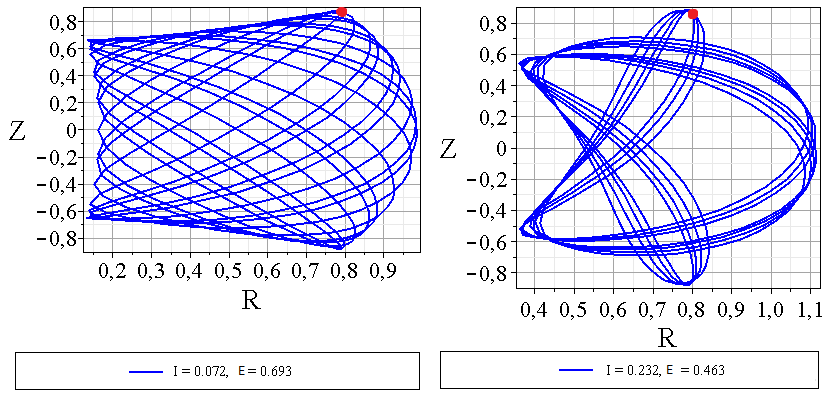
\includegraphics[width=\linewidth]{D:/diploma/tex/2/res/dual1.png}
\end{minipage}
\caption{Проекции орбиты на сопутствующую плоскость в модели (2), (3). Значения интегралов площадей и энергии $I_1 = 0.072$, $E_1 = 0.69$ (справа), $I_2 = 0.232$, $E_2 = 0.46$(слева).}
\end{figure}

\begin{figure}[H]
\centering
\begin{minipage}[t]{1\textwidth}
\centering
\includegraphics[width=\linewidth]{D:/diploma/tex/2/res/dual2.png}
\end{minipage}
\caption{Проекции орбиты на сопутствующую плоскость в модели (2), (3). Значения интегралов площадей и энергии $I_1 = 0.24$, $E_1 = 0.65$ (справа), $I_2 = 0.312$, $E_2 = 0.43$(слева).}
\end{figure}
}
~\par

Проварьируем значения параметров, выбирая те из них, которые порождают физически корректную модель, и посмотрим, как изменятся орбиты. Большинство вычисленных орбит оказываются ящичными~(см.~рис.~\ref{orbits:1}).

{
\begin{figure}[H]
\centering
\begin{minipage}[t]{0.8\textwidth}
\centering
\includegraphics[width=\linewidth]{D:/diploma/tex/2/res/alpha.png}
\end{minipage}
\caption{Сравнение орбит при различных значениях параметра $\alpha$}\label{orbits:1}
\end{figure}
}

{
\begin{figure}[H]
\centering
\begin{minipage}[t]{0.8\textwidth}
\centering
\includegraphics[width=\linewidth]{D:/diploma/tex/2/res/p.png}
\end{minipage}
\caption{Сравнение орбит при различных значениях параметра $p$}\label{orbits:2}
\end{figure}
}

{
\begin{figure}[H]
\centering
\begin{minipage}[t]{0.8\textwidth}
\centering
\includegraphics[width=\linewidth]{D:/diploma/tex/2/res/epsilon.png}
\end{minipage}
\caption{Сравнение орбит при различных значениях параметра $\varepsilon$}\label{orbits:3}
\end{figure}
}
Из рисунков~\ref{orbits:1},~\ref{orbits:2},~\ref{orbits:3} видно, что морфология орбит существенно не меняется, пробная звезда просто движется в более или менее широкой области.
~\par
Во второй главе была рассмотрена задача Коши, решая которую мы получаем орбиты пробной звезды в рассматриваемой модели. Выбран метод численного интегрирования Рунге-Кутта-Фельберга для того, чтоб получить достаточно точные орбиты. Построена диаграмма Линдблада для выбора начальных условий, а так же на ней отмечены используемые начальные условия, для которых решается поставленная задача Коши. Построены орбиты пробных звезд (около 1000, некоторые наиболее интересные отмечены в работе) и показано влияние на них параметров модели. Сделано заключение, что существенно параметры модели не изменяют морфологию орбит.